\documentclass{article}
\usepackage{fontspec}
\usepackage{geometry}
\usepackage[table]{xcolor}
\usepackage{tabularx}
\usepackage{graphicx}
\usepackage{mathtools}
\usepackage[clean]{svg}
\usepackage[bottom]{footmisc}

\usepackage{listings}
\usepackage{color}
\renewcommand\lstlistingname{Quelltext} % Change language of section name
\lstset{ % General setup for the package
    language=SQL,
    basicstyle=\small\sffamily,
    numbers=left,
     numberstyle=\tiny,
    frame=tb,
    tabsize=4,
    columns=fixed,
    showstringspaces=false,
    showtabs=false,
    keepspaces,
    commentstyle=\color{red},
    keywordstyle=\color{blue}
}

\geometry{
a4paper,
total = {170mm, 240mm},
left = 20mm,
top = 20mm,
}

\setlength{\parindent}{0em}
\setlength{\parskip}{0.5em}



\author{Alessandro Massarenti, Filippo Zonta Rocha}
\title{
Gestionale servizi portuali\\
\small Progetto di basi di dati
}
\date{a.a. 2020/2021}

\begin{document}
\setmainfont{Arial}

\maketitle

\subsection{Abstract}

%quesito
Moltissime imbarcazioni ogni giorno navigano i mari di tutto il mondo, e dopo giorni, a volte settimane, di navigazione è importante per gli equipaggi di questi scafi da diporto riposare in un posto sicuro, accogliente ed efficiente.

%soluzione
Per rispondere a questa necessità numerose località di mare, turistiche e non, si sono dotate di piccoli porticcioli in luoghi strategici, mirati a proteggere e sistemare le imbarcazioni, a semplificare le pratiche burocratiche e a connettere le persone al mare.

%in dettaglio
Questi porticcioli si chiamano \textbf{marina}. I marina devono soddisfare molti requisiti e hanno molte operazioni che possono essere migliorate e coadiuvate da un sistema informativo, molte operazioni sono infatti ripetitive, lavorano su grosse quantità di dati o sono richieste ad orari anomali. Relativamente all'ultima questione infatti, non tutte le imbarcazioni entrano in porto come in hotel in degli orari prestabiliti. Un numero significativo di imbarcazioni arriva nei marina agli orari più disparati, e non sempre è possibile avere tutto il personale disponibile per gestire le richieste.


\section{Analisi dei requisiti}
\subsection{Descrizione testuale}
Si vuole realizzare una base di dati per l'applicazione \textit{Gestionale servizi del diporto} che dovrà gestire tutti i dati relativi ad le imbarcazioni che vi sosteranno, i servizi offerti e i dati relativi ai clienti.

Ogni marina solitamente contiene da 50 fino ad anche 500 \textbf{posti barca} con un commisurato traffico di imbarcazioni, persone e quindi informazioni. Alcuni dei clienti del marina sono occasionali, ad esempio persone che effettuano crociere e bazzicano di porto in porto; Altri clienti sono abituali e tengono ormeggiate le loro imbarcazioni nel marina per molti mesi all'anno se non addirittura a tempo indeterminato. Si vorrà poi sapere da quanto tempo un posto barca appartiene ad una persona.

Ognuno di questi marina è caratterizzato da un indirizzo, \textit{un nome}, e \textit{le coordinate geografiche} a cui i naviganti possono dirigere per raggiungerlo. Esso possiede inoltre una quantità più o meno varia di moli\footnote{Sinonimo di posto barca} di cui si vuole tenere traccia l'occupazione nel tempo per fini statistici\footnote{Quando e per quanto}. per ogni molo sono registrate le dimensioni(Molto importanti, poiché solo le imbarcazioni più piccole di queste dimensioni potranno ormeggiare in questo molo), gli allacciamenti\footnote{Si intendono allacciamenti idrici, elettrici, di aria compressa} e lo stato di occupazione.

Gli allacciamenti hanno un nome, un'unità di misura ed un costo unitario.

Relativamente agli allacciamenti ne vengono anche registrati i consumi da parte di ogni cliente, come procedura interna del marina viene fatta una lettura del contatore all'arrivo dell'imbarcazione ed una lettura del contatore alla partenza della stessa. Se l'imbarcazione non ha una data di prevista partenza, ad esempio un cliente che ormeggia la sua imbarcazione a tempo indefinito la lettura viene fatta mensilmente e registrata, la quantità da pagare mensilmente viene quindi fatturata al cliente e viene registrato se la fattura è stata pagata oppure no.

%per ogni sosta di un'imbarcazione in un molo si vuole memorizzare la data in cui l'imbarcazione è arrivata e la data in cui l'imbarcazione è partita. 

%Degli allacciamenti è importante il tipo di allacciamento, il prezzo unitario e l'unità di misura.

Nel marina sosteranno le \textbf{imbarcazioni}, queste imbarcazioni sosteranno nel tempo in più moli differenti. Chiaramente i moli saranno nel tempo utilizzati da più imbarcazioni(o anche da nessuna(ad esempio un marina appena inaugurato)).

Di ogni \textbf{imbarcazione} vengono registrati codice internazionale, la bandiera battuta,l'armatore, il capitano le dimensioni, il numero di posti letto e se è presente anche il nome. Queste informazioni vengono memorizzate assieme ai dati dei clienti per onorare gli obblighi di registrazione portuale.

I clienti sono coloro che ormeggiano un'imbarcazione all'interno del marina e di loro ne viene salvato il nome, il cognome, il codice fiscale, gli eventuali contatti, la residenza, la cittadinanza, la data di nascita.

Ogni cliente può quindi prenotare un molo del marina preventivamente. Ogni \textbf{prenotazione} è caratterizzata da una data prevista di arrivo, una data prevista di partenza, l'imbarcazione interessata, ed il cliente prenotante.

%Per controllare se un posto è disponibile bisogna quindi controllare se il molo è disponibile e inoltre se esistono già delle prenotazioni per quelle date. In realtà le prenotazioni non sono obbligatoriamente associate ad un molo, ma sono associate alle dimensioni. Infatti è importante trovare il best match tra imbarcazioni e moli, ma non serve che un molo sia forzatamente prenotato per un'imbarcazione.

Il marina offre una serie di servizi utili ai naviganti\footnote{Ad esempio lavanderie a gettoni, ristoranti, cantieri} . Ogni servizio è caratterizzato da un nome unico per ogni marina e gli orari di apertura e chiusura.

Ogni servizio è amministrato da un \textbf{addetto} del quale ci interessa la data di inizio contratto e la fine. Se la fine non è segnata allora lavorerà li a tempo indeterminato.

Come terzo ed ultimo metodo di sostentamento il marina offre anche dei \textbf{corsi}, questi corsi utilizzano a volte le imbarcazioni messe a disposizione da alcune persone e ne viene registrato il nome, il prezzo per la partecipazione, la data di inizio e la data di fine del corso. Esisteranno quindi dei clienti senza imbarcazione ma che partecipano ad uno dei corsi offerti dal marina.
 
 
%%%%%%%%%%%%
%Il conto di un cliente in fine equivale alla somma di tutti i servizi di cui ha usufruito e dei giorni in cui ha sostato.
%%%%%%%%%%%%

\subsection{Glossario dei termini}

\begin{center}
    \begin{tabularx}{\textwidth}{|p{2.4cm}|p{8cm}|p{2.4cm}|X|}
        \hline
        \textbf{Entità} & \textbf{Descrizione} & \textbf{Sinonimi} & \textbf{collegamenti} \\
        \hline
        Marina & Il luogo in cui si trovano tutte le imbarcazioni ed i servizi  & area portuale & molo, servizio, imbarcazione\\
        
        \hline
        Imbarcazione & Il mezzo di trasporto parcheggiato nei moli & barca & persona, molo\\
        
        \hline
        Molo & Il luogo in cui le imbarcazioni riposano & posto barca, ormeggio & persona, imbarcazione\\
        
        \hline
        Cliente& Persona che possiede un'imbarcazione ormeggiata nel marina & armatore & imbarcazione\\
        
        \hline
        Prenotazione &&&molo, cliente \\
        
        \hline
        Servizio &&&Marina \\
        
        \hline
        Addetto & Persona con responsabilità relative ad un servizio & & servizio \\
        
        \hline
        Allacciamento & Un servizio consumabile tipo acqua, elettricità disponibile ad un molo& & molo\\
        \hline
        Corso & & &marina, imbarcazione, cliente\\
        \hline
        Fattura &&& cliente, consumo\\
        \hline
        Consumo & La lettura di un contatore degli allacciamenti presenti ai moli.& & fattura, cliente, molo\\
        \hline
    \end{tabularx}
\end{center}

\subsection{Strutturazione dei requisiti}

\begin{center}
    \begin{tabularx}{\textwidth}{|X|}
        \hline
        \rowcolor{gray!30}
        \multicolumn{1}{|c|}{\textbf{Frasi relative a Marina}}\\
        \hline
        Ogni marina solitamente contiene da 50 fino ad anche 500posti barca. \\
        
        Ognuno di questi marina è caratterizzato da un indirizzo, \textit{un nome}, e \textit{le coordinate geografiche} a cui i naviganti possono dirigere per raggiungerlo. Esso possiede inoltre una quantità più o meno varia di moli\\
        
        Nel marina sosteranno le imbarcazioni,queste imbarcazioni sosteranno nel tempo in più moli differenti.\\
        \hline
    \end{tabularx}
\end{center}

\begin{center}
    \begin{tabularx}{\textwidth}{|X|}
        \hline
        \rowcolor{gray!30}
        \multicolumn{1}{|c|}{\textbf{Frasi relative a Imbarcazione}}\\
        \hline
        queste imbarcazioni sosteranno nel tempo in più moli differenti.\\
        Di ogni \textbf{imbarcazione} vengono registrati codice internazionale, la bandiera battuta,l'armatore, il capitano le dimensioni, il numero di posti letto e se è presente anche il nome. Queste informazioni vengono memorizzate assieme ai dati dei clienti per onorare gli obblighi di registrazione portuale.\\
        \hline
    \end{tabularx}
\end{center}

\begin{center}
    \begin{tabularx}{\textwidth}{|X|}
        \hline
        \rowcolor{gray!30}
        \multicolumn{1}{|c|}{\textbf{Frasi relative a Molo}}\\
        \hline
        moli di cui si vuole tenere traccia l’occupazione nel tempo per fini statistici. per ogni molo sono registrate le dimensioni(Molto importanti, poiché solo le imbarcazioni più piccole di queste dimensioni potranno ormeggiare in questo molo),gli allacciamenti e lo stato di occupazione.\\
        \hline
    \end{tabularx}
\end{center}

\begin{center}
    \begin{tabularx}{\textwidth}{|X|}
        \hline
        \rowcolor{gray!30}
        \multicolumn{1}{|c|}{\textbf{Frasi relative a Cliente}}\\
        \hline
        Alcuni dei clienti del marina sono occasionali, ad esempio persone che effettuano crociere e bazzicano di porto in porto; Altri clienti sono abituali e tengono ormeggiate le loro imbarcazioni nel marina per molti mesi all'anno se non addirittura a tempo indeterminato.\\
        
        I clienti sono coloro che ormeggiano un'imbarcazione all'interno del marina e di loro ne viene salvato il nome, il cognome, il codice fiscale, gli eventuali contatti, la residenza, la cittadinanza, la data di nascita.\\

Ogni cliente può quindi prenotare un molo del marina preventivamente.\\
        \hline
    \end{tabularx}
\end{center}

\begin{center}
    \begin{tabularx}{\textwidth}{|X|}
        \hline
        \rowcolor{gray!30}
        \multicolumn{1}{|c|}{\textbf{Frasi relative a Prenotazione}}\\
        \hline
        Ogni \textbf{prenotazione} è caratterizzata da una data prevista di arrivo, una data prevista di partenza, l'imbarcazione interessata, ed il cliente prenotante.\\
        \hline
    \end{tabularx}
\end{center}

\begin{center}
    \begin{tabularx}{\textwidth}{|X|}
        \hline
        \rowcolor{gray!30}
        \multicolumn{1}{|c|}{\textbf{Frasi relative a Servizio}}\\
        \hline
        Il marina offre una serie di servizi utili ai naviganti\footnote{Ad esempio lavanderie a gettoni, ristoranti, cantieri} . Ogni servizio è caratterizzato da un nome unico per ogni marina e gli orari di apertura e chiusura.\\
        
        Ogni servizio è amministrato da un \textbf{addetto} \\
        \hline
    \end{tabularx}
\end{center}

\begin{center}
    \begin{tabularx}{\textwidth}{|X|}
        \hline
        \rowcolor{gray!30}
        \multicolumn{1}{|c|}{\textbf{Frasi relative a Addetto}}\\
        \hline
        un \textbf{addetto} del quale ci interessa la data di inizio contratto e la fine. Se la fine non è segnata allora lavorerà li a tempo indeterminato.\\
        \hline
    \end{tabularx}
\end{center}

\begin{center}
    \begin{tabularx}{\textwidth}{|X|}
        \hline
        \rowcolor{gray!30}
        \multicolumn{1}{|c|}{\textbf{Frasi relative a Allacciamento}}\\
        \hline
        Gli allacciamenti hanno un nome, un'unità di misura ed un costo unitario.\\
        Relativamente agli allacciamenti ne vengono anche registrati i consumi da parte di ogni cliente\\
        \hline
    \end{tabularx}
\end{center}


\begin{center}
    \begin{tabularx}{\textwidth}{|X|}
        \hline
        \rowcolor{gray!30}
        \multicolumn{1}{|c|}{\textbf{Frasi relative a Corso}}\\
        \hline
        Questi corsi utilizzano a volte le imbarcazioni messe a disposizione da alcune persone e ne viene registrato il nome, il prezzo per la partecipazione, la data di inizio e la data di fine del corso. Esisteranno quindi dei clienti senza imbarcazione ma che partecipano ad uno dei corsi offerti dal marina.\\
        \hline
    \end{tabularx}
\end{center}

\begin{center}
    \begin{tabularx}{\textwidth}{|X|}
        \hline
        \rowcolor{gray!30}
        \multicolumn{1}{|c|}{\textbf{Frasi relative a Fattura}}\\
        \hline
        la quantità da pagare mensilmente viene quindi fatturata al cliente e viene registrato se la fattura è stata pagata oppure no.\\
        \hline
    \end{tabularx}
\end{center}

\begin{center}
    \begin{tabularx}{\textwidth}{|X|}
        \hline
        \rowcolor{gray!30}
        \multicolumn{1}{|c|}{\textbf{Frasi relative a Consumo}}\\
        \hline
        vengono anche registrati i consumi da parte di ogni cliente, come procedura interna del marina viene fatta una lettura del contatore all'arrivo dell'imbarcazione ed una lettura del contatore alla partenza della stessa. Se l'imbarcazione non ha una data di prevista partenza, ad esempio un cliente che ormeggia la sua imbarcazione a tempo indefinito la lettura viene fatta mensilmente e registrata.\\
        \hline
    \end{tabularx}
\end{center}

\subsection{Operazioni tipiche}
Contando che ad un marina appartengono dai 50 ai 500 moli e una delle aziende o associazioni che utilizzerà l'applicativo potrebbe possedere da 1 a 5 marina in media le operazioni effettuate nel marina con annessa frequenza sono le seguenti.
\begin{center}
    \begin{tabularx}{\textwidth}{|p{90mm}|X|}
        \hline
        \rowcolor{gray!30}
        \textbf{Operazione} & \textbf{Frequenza}\\
        \hline
        1. Stampa della fattura di pagamento del cliente & 40 volte al giorno\\
        \hline
        2. Controllo dei posti disponibili per una certa imbarcazione(Controllo delle dimensioni)& 40 volte al giorno\\
        \hline
        3. Organizzazione di un corso & 30 volte l'anno\\
        \hline
        4. Cambio dell'addetto ad un servizio & 1-2 volte ogni due anni\\
        \hline
        5. Prenotazioni di posti barca & 30-50 volte al giorno\\
        \hline
        6. Arrivo di un'imbarcazione in uno dei marina & 30-40 volte al giorno\\
        \hline
        7. Espletamento degli obblighi doganali & 140 volte a settimana\\
        \hline
    \end{tabularx}
\end{center}

\section{Progettazione concettuale}

\subsection{Analisi delle entità}

%Imbarcazione
\begin{center}
    \begin{tabularx}{\textwidth}{|l|l|l|X|}
        \hline
        \rowcolor{gray!30}
        \multicolumn{4}{|c|}{\textbf{Imbarcazione}}\\
        \hline
        Codice internazionale & VARCHAR & Identifica univocamente un'imbarcazione nel mondo & Chiave\\
        \hline
        Nome & VARCHAR & \multicolumn{2}{l|}{Il nome dell'imbarcazione} \\
        \hline
        QtPostiLetto & INTEGER & \multicolumn{2}{l|}{La quantità di posti letto dell'imbarcazione} \\
        \hline
        Nome del capitano & VARCHAR & \multicolumn{2}{l|}{Il nome del capitano} \\
        \hline
        Bandiera & VARCHAR & \multicolumn{2}{l|}{Nome dello stato di cui batte bandiera l'imbarcazione} \\
        \hline
        Dimensioni &  & \multicolumn{2}{l|}{Attributo composto: Pescaggio, Larghezza, LOA} \\
        \hline
        Pescaggio & DECIMAL & \multicolumn{2}{l|}{La misura del punto più in profondità dell'imbarcazione} \\
        \hline
        Larghezza & DECIMAL & \multicolumn{2}{l|}{La misura della larghezza al baglio massimo dell'imbarcazione} \\
        \hline
        LOA & DECIMAL & \multicolumn{2}{l|}{La misura della lunghezza fuoritutto dell'imbarcazione} \\
        \hline
    \end{tabularx}
\end{center}

%Molo
\begin{center}
    \begin{tabularx}{\textwidth}{|l|l|l|X|}
        \hline
        \rowcolor{gray!30}
        \multicolumn{4}{|c|}{\textbf{Molo}}\\

        \hline
        Numero molo & INTEGER & Identifica univocamente un molo & Chiave\\
        \hline
        Stato di occupazione & BOOLEAN &\multicolumn{2}{l|}{ Lo stato di occupazione del molo}\\
        \hline
        Dimensioni &  & \multicolumn{2}{l|}{Attributo composto: Profondità minima, Larghezza, Lunghezza} \\
        \hline
        Profondità minima & DECIMAL & \multicolumn{2}{l|}{La profondità misurata alla più bassa marea sizigiale} \\
        \hline
        Larghezza & DECIMAL & \multicolumn{2}{l|}{La misura della larghezza del molo} \\
        \hline
        Lunghezza & DECIMAL & \multicolumn{2}{l|}{La misura della lunghezza del molo} \\
        \hline
    \end{tabularx}
\end{center}

%servizio
\begin{center}
    \begin{tabularx}{\textwidth}{|l|l|l|X|}
        \hline
        \rowcolor{gray!30}
        \multicolumn{4}{|c|}{\textbf{Servizio}}\\
        \hline
        Nome & VARCHAR & Il nome del servizio & Chiave \\
        \hline
    \end{tabularx}
\end{center}


%Addetto
\begin{center}
    \begin{tabularx}{\textwidth}{|l|l|l|X|}
        \hline
        \rowcolor{gray!30}
        \multicolumn{4}{|c|}{\textbf{Addetto}}\\
        \hline
        Servizio & VARCHAR & È il servizio in cui lavora & \multirow{2}{*}{Chiave}\\
        \hhline{---}
        DataInizioContratto & DATE & È la data in cui il contratto è iniziat& \\
        \hline
        DataFineContratto & DATE &\multicolumn{2}{l|}{ È la data in cui il contratto è finito o finirà.}\\
        \hline
    \end{tabularx}
\end{center}

%Cliente
\begin{center}
    \begin{tabularx}{\textwidth}{|l|l|X|}
        \hline
        \rowcolor{gray!30}
        \multicolumn{3}{|c|}{\textbf{Cliente}}\\
        \hline
        Cittadinanza & VARCHAR & Lo stato di cui il cliente è cittadino\\
        \hline
        Residenza & VARCHAR & La città in cui il cliente è residente \\
        \hline
    \end{tabularx}
\end{center}

%Cliente occasionale
\begin{center}
    \begin{tabularx}{\textwidth}{|l|l|X|}
        \hline
        \rowcolor{gray!30}
        \multicolumn{3}{|c|}{\textbf{Cliente occasionale}}\\
        \hline
        Quantità di soste & INTEGER & Il numero di soste che il cliente ha effettuato presso la struttura \\
        \hline
    \end{tabularx}
\end{center}

%Cliente abituale
\begin{center}
    \begin{tabularx}{\textwidth}{|l|l|X|}
        \hline
        \rowcolor{gray!30}
        \multicolumn{3}{|c|}{\textbf{Cliente abituale}}\\
        \hline
        Sconto personale & DECIMAL & Lo sconto percentuale applicato alle sue fatture \\
        \hline
    \end{tabularx}
\end{center}

%Persona
\begin{center}
    \begin{tabularx}{\textwidth}{|l|l|l|X|}
        \hline
        \rowcolor{gray!30}
        \multicolumn{4}{|c|}{\textbf{Persona}}\\
        \hline
        CF & VARCHAR & Identifica univocamente una persona & Chiave \\
        \hline
        Nome & VARCHAR & \multicolumn{2}{l|}{Il nome della persona} \\
        \hline
        Cognome & VARCHAR & \multicolumn{2}{l|}{Il cognome della persona} \\
        \hline
        DataNascita & DATE & \multicolumn{2}{l|}{La data di nascita della persona} \\
        \hline
        Contatto & VARCHAR & \multicolumn{2}{l|}{I contatti della persona(multi-valore)} \\
        \hline
    \end{tabularx}
\end{center}

%Prenotazione
\begin{center}
    \begin{tabularx}{\textwidth}{|l|l|l|X|}
        \hline
        \rowcolor{gray!30}
        \multicolumn{4}{|c|}{\textbf{Prenotazione}}\\
        \hline
        CF & VARCHAR & Il codice fiscale del cliente prenotante & \multirow{3}{*}{Chiave}\\
        \hhline{---}
        Molo & INTEGER & Il molo prenotante &\\
        \hhline{---}
        Previsione arrivo & DATE & La data in cui si prevede il cliente arrivo &\\
        \hline
        Previsione partenza & DATE & \multicolumn{2}{l|}{La data in cui si prevede il cliente parta}\\
        \hline
        Stato di arrivo & BOOLEAN & \multicolumn{2}{l|}{Il cliente ha trasformato oppure no la prenotazione in sosta}\\
        \hline
    \end{tabularx}
\end{center}

%Sosta
\begin{center}
    \begin{tabularx}{\textwidth}{|l|l|l|X|}
        \hline
        \rowcolor{gray!30}
        \multicolumn{4}{|c|}{\textbf{Sosta}}\\
        Imbarcazione & VARCHAR & Il codice internazionale dell'imbarcazione & \multirow{3}{*}{Chiave}\\
        \hhline{---}
        Molo & INTEGER & Il molo della sosta &\\
        \hhline{---}
        Data arrivo & TIMESTAMP & Data in cui l'imbarcazione ha ormeggiato & \\
        \hline
        Data partenza & TIMESTAMP & \multicolumn{2}{l|}{Data in cui l'imbarcazione ha sciolto gli ormeggi} \\
        \hline
    \end{tabularx}
\end{center}

%Allacciamento
\begin{center}
    \begin{tabularx}{\textwidth}{|l|l|l|X|}
        \hline
        \rowcolor{gray!30}
        \multicolumn{4}{|c|}{\textbf{Allacciamento}}\\
        \hline
        Nome & VARCHAR & Il nome che identifica la tipologia di allacciamento &Chiave\\
        \hline
        Prezzo unitario & DECIMAL & \multicolumn{2}{l|}{Il prezzo unitario dell'allacciamento}\\
        \hline
        Unità di misura & VARCHAR & \multicolumn{2}{l|}{L'unità di misura utilizzata per conteggiarne il consumo}\\
        \hline
    \end{tabularx}
\end{center}

%Periodo di apertura
\begin{center}
    \begin{tabularx}{\textwidth}{|l|l|l|X|}
        \hline
        \rowcolor{gray!30}
        \multicolumn{4}{|c|}{\textbf{Periodo di apertura}}\\
        \hline
        Giorno di apertura & CHAR(3) & Giorno a cui si riferisce l'orario di apertura &\multirow{3}{*}{Chiave}\\
        \hhline{---}
        Orario di apertura & TIME & Orario a cui il servizio apre nel giorno & \\
        \hhline{---}
        Orario di chiusura & TIME & Orario a cui il servizio cudehi nel giorno & \\
        \hline
    \end{tabularx}
\end{center}

%Consumo
\begin{center}
    \begin{tabularx}{\textwidth}{|l|l|l|X|}
        \hline
        \rowcolor{gray!30}
        \multicolumn{4}{|c|}{\textbf{Consumo}}\\

        \hline
        Cliente & VARCHAR & Cliente consumante & \multirow{3}{*}{Chiave} \\
        \hhline{---}
        Allacciamento & VARCHAR & il tipo di allacciamento consumato &\\
        \hhline{---}
        Data inizio lettura & TIMESTAMP & Momento dell'inizio del conteggio & \\
        \hline
        Data fine lettura & TIMESTAMP & \multicolumn{2}{l|}{Momento della fine del conteggio}\\
        \hline
        Quantità consumata & DECIMAL & \multicolumn{2}{l|}{La quantità consumata nel periodo} \\
        \hline
    \end{tabularx}
\end{center}

%Fattura
\begin{center}
    \begin{tabularx}{\textwidth}{|l|l|l|X|}
        \hline
        \rowcolor{gray!30}
        \multicolumn{4}{|c|}{\textbf{Fattura}}\\
        \hline

        \hline
        Cliente & VARCHAR & Cliente ricevente & \multirow{2}{*}{Chiave} \\
        \hhline{---}
        Data scadenza & TIMESTAMP & Identifica la scadenza della fattura & \\
        \hline
        Pagato & TIMESTAMP & \multicolumn{2}{l|}{Identifica quando è stata pagata e lo stato del pagamento della fattura} \\
        \hline
    \end{tabularx}
\end{center}


\subsection{Generalizzazioni}

\begin{itemize}
    \item Persona è generalizzazione parziale esclusiva di Addetto;
    \item Persona è generalizzazione parziale esclusiva di Cliente;
    \item Cliente è generalizzazione totale esclusiva di cliente abituale e cliente occasionale;
\end{itemize}

\subsection{Analisi delle relazioni e delle cardinalità}

\begin{itemize}
    
    \item Molo - Allacciamento: \textbf{Fornitura}
    \begin{itemize}
        \item Un Molo possiede più allacciamenti o nessuno (0,N);
        \item Un allacciamento può essere posseduto da più moli o da nessuno(0,N);
    \end{itemize}

    \item Consumo - Allacciamento: \textbf{Utilizzo}
    \begin{itemize}
        \item Un consumo utilizza uno e un solo allacciamento(1,1);
        \item Un allacciamento può essere utilizzato da 0 a molti consumi(0,N);
    \end{itemize}

    \item Consumo - Fattura: \textbf{Riga fattura consumo}
    \begin{itemize}
        \item Un consumo è riga di una o nessuna fattura(0,1);
        \item Una fattura ha da 0 a molte righe relative ai consumi(0,N);
    \end{itemize}

    \item Sosta - Fattura: \textbf{Riga fattura sosta}
    \begin{itemize}
        \item Una sosta è riga di una o nessuna fattura(0,1);
        \item Una fattura ha da 0 a molte righe relative alle soste (0,N);
    \end{itemize}

    \item Fattura - Cliente: \textbf{Destinatario fattura}
    \begin{itemize}
        \item Una fattura è destinata ad uno e un solo cliente(0,1);
        \item Un cliente può avere da 0 a molte fatture destinategli(0,N);
    \end{itemize}

    \item Addetto - Servizio: \textbf{Gestione}
    \begin{itemize}
        \item Un addetto gestisce uno e un solo servizio (1,1);
        \item Un servizio è gestito da un addetto o da nessuno (0,1);
    \end{itemize}

    \item Servizio - Periodo apertura: \textbf{Apertura}
    \begin{itemize}
        \item Un servizio ha da uno a molte aperture(1,N);
        \item Periodo di apetura definisce aperte da uno a molti servizi (1,N);
    \end{itemize}

    \item Consumo - Cliente: \textbf{Consumazione}
    \begin{itemize}
        \item Un Cliente effettua da 0 a molte consumazioni di consumazione(0,N);
        \item Un consumo è consumazione di uno e un solo cliente (1,1);
    \end{itemize}

    \item Prenotazione - Molo: \textbf{Riserve}
    \begin{itemize}
        \item Una prenotazione Riserva uno e un solo molo (1,1);
        \item Un molo può essere riservato da più prenotazioni o da nessuna (0,N);
    \end{itemize}

    \item Cliente - Imbarcazione: \textbf{Proprietà}
    \begin{itemize}
        \item Un cliente può possedere più imbarcazioni(Almeno una) (1,N);
        \item Un imbarcazione è posseduta da una e una sola una persona oppure da nessuno\footnote{Barca abbandonata}(0,1);
    \end{itemize}
    
    \item Cliente - Prenotazione: \textbf{Prenotazioni effettuate}
    \begin{itemize}
        \item Un cliente può aver effettuato da 0 a molte prenotazioni(0,N);
        \item Una prenotazione può essere stata effettuata al massimo da un cliente (1,1);
    \end{itemize}

    \item Molo - Sosta: \textbf{M\_S}
    \begin{itemize}
        \item Un molo può accogliere da 0 a molte soste(0,N);
        \item Una sosta è relativa a uno e un solo molo(1,1);
    \end{itemize}

    \item Sosta - Imbarcazione: \textbf{S\_I}
    \begin{itemize}
        \item Una sosta è relativa ad una e una sola imbarcazione(1,1);
        \item Un imbarcazione può sostare da 0 a molte volte (0,N);
    \end{itemize}
    
\end{itemize}

\subsection{Schema ER concettuale}
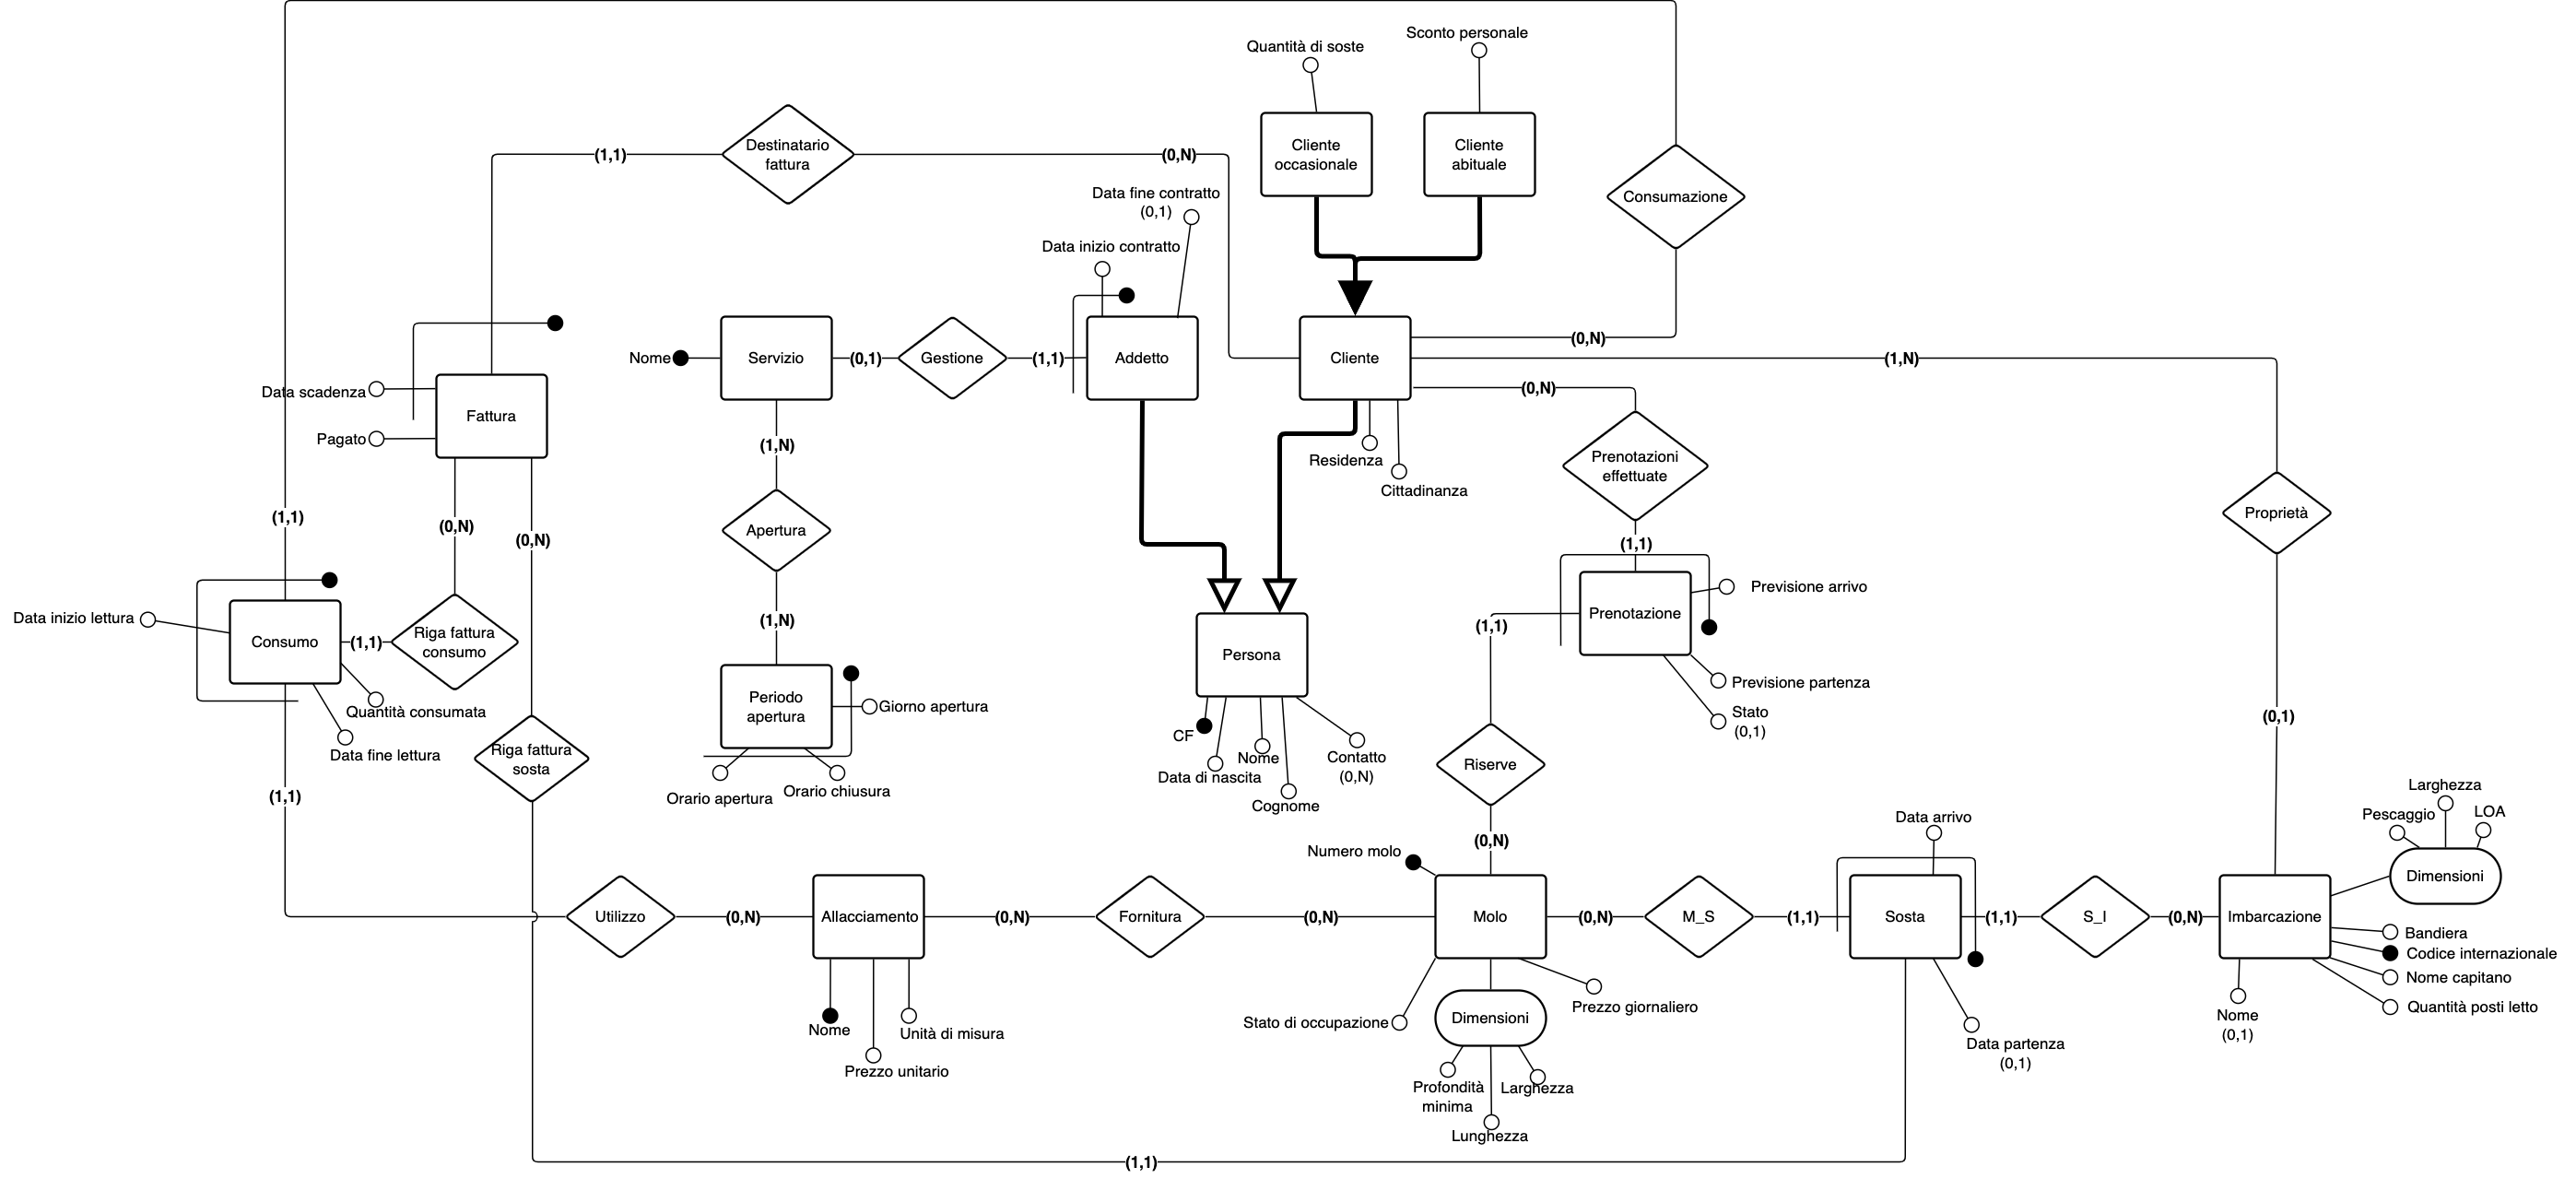
\includegraphics[width=\textwidth]{img/erconcettuale.png}

\subsubsection{Vincoli non rappresentabili nello schema Relazionale}

\begin{center}
    \begin{tabularx}{\textwidth}{|p{30mm}|X|}
        \hline
        \rowcolor{gray!30}
        \textbf{Entità / Relazione} & \textbf{Vincolo}\\
        \hline
        Molo & Lo stato di occupazione deve essere coerente con la sosta\\
        \hline

        Periodo di apertura & orario di chiusura deve essere postumo all'orario di apertura \\
        \hline

        Fattura & deve essere presente almeno una linea di consumo o una linea di sosta\\
        \hline

        Prenotazione & La previsione della partenza deve essere postuma alla previsione dell'arrivo\\
        \hline

        Prenotazione & Un molo non può essere prenotato nello stesso momento da due persone differenti e non può essere prenotato se c'è già una barca in sosta\\
        \hline

        Sosta & La data di partenza deve essere postuma alla data di arrivo\\

        \hline
        Sosta & Un molo non può essere utilizzato se è già occupato o è prenotato e un'imbarcazione non può occupare due moli contemporaneamente\\

        \hline
    \end{tabularx}
\end{center}

\section{Progettazione logica}

\subsection{Analisi delle ridondanze}
Nello schema concettuale possiamo individuare stato di occupazione che è attributo di molo e deducibile dalla relazione sosta, la quale presenta l'attributo data di arrivo e data di partenza.

Le operazioni coinvolte sono la numero 3 e la numero 6 che presentano una frequenza di 40 volte al giorno e 30-40 volte ogni giorno.

Si procede alla valutazione del costo totale in termini di accessi nel caso di ridondanza e di assenza di essa.

\begin{center}
    \begin{tabularx}{\textwidth}{|p{90mm}|X|}
        \hline
        \rowcolor{gray!30}
        \textbf{Operazione} & \textbf{Frequenza}\\
        \hline
        3. Controllo dei posti disponibili per una certa imbarcazione(Controllo delle dimensioni)& 40 volte al giorno\\
        \hline
        6. Arrivo di un'imbarcazione nel marina & 30-40 volte al giorno\\
        \hline
    \end{tabularx}
\end{center}

Ci riferiremo per i nostri calcoli a dei volumi plausibili nella vita della base di dati. I moli non variano particolarmente di numero, le imbarcazioni vengono registrate al loro primo accesso e le soste aumentano ogni giorno. Mediamente un'imbarcazione sosta 2,7 volte in un molo.

\begin{center}
    \begin{tabularx}{\textwidth}{|X|X|X|}
        \hline
        \rowcolor{gray!30}
        \textbf{Concetto} & \textbf{Tipo} & \textbf{Volume}\\
        \hline
        Molo & ENTITÀ & 250\\
        \hline
        Imbarcazione & ENTITÀ & 5000\\
        \hline
        Sosta & ENTITÀ & 13500\\ % Contando che ogni imbarcazione sosta in media due volte per molo.
        \hline
        M\_S & RELAZIONE & 13500\\ % Contando che ogni imbarcazione sosta in media due volte per molo.
        \hline
    \end{tabularx}
\end{center}

\paragraph{operazione 3}

\begin{center}
    \begin{minipage}{.48\linewidth}
        \begin{tabularx}{\linewidth}{|X|l|l|l|}
            \hline
            \rowcolor{gray!30}
            \multicolumn{4}{|c|}{\textbf{Con ridondanza}}\\
            \hline
            \rowcolor{gray!15}
            Concetto & Costrutto & Accessi & Tipo\\
            \hline
            Molo & E & 250 & L\\
            \hline
        \end{tabularx}
    \end{minipage}
    \begin{minipage}{.48\linewidth}
        \begin{tabularx}{\linewidth}{|X|l|l|l|}
            \hline
            \rowcolor{gray!30}
            \multicolumn{4}{|c|}{\textbf{Senza ridondanza}}\\
            \hline
            \rowcolor{gray!15}
            Concetto & Costrutto & Accessi & Tipo\\
            \hline
            Sosta & E & 13500 & L\\
            \hline
            M\_S & R & 13500 & L\\
            \hline
            Molo & E & 250 & L\\
            \hline
        \end{tabularx}
    \end{minipage}
\end{center}

\underline{Con ridondanza}
\begin{itemize}
    \item Totale accessi(Solo in lettura): $250\xrightarrow{*40} 10000$
\end{itemize}

\underline{Senza ridondanza}
\begin{itemize}
    \item Totale accessi(Solo in lettura): $250+13500+13500 = 27250 \xrightarrow{*40} 1090000$ Giornalieri
\end{itemize}

\paragraph{operazione 6}

Assumo che l'imbarcazione sia già presente perché l'esserci o non esserci non cambia il calcolo della ridondanza.

\begin{center}
\begin{tabularx}{\linewidth}{|X|}
    \hline
    \rowcolor{gray!30}
    \multicolumn{1}{|c|}{\textbf{Operazioni principali}}\\
    \hline
    Cerco l'imbarcazione\\
    \hline
    Cerco i moli disponibili\\
    \hline
    Confronto le dimensioni dell'imbarcazione con i moli disponibili\\
    \hline
    Scrivo la sosta\\
    \hline
\end{tabularx}
\end{center}


\begin{center}
    \begin{minipage}{.48\linewidth}
        \begin{tabularx}{\linewidth}{|X|l|l|l|}
            \hline
            \rowcolor{gray!30}
            \multicolumn{4}{|c|}{\textbf{Con ridondanza}}\\
            \hline
            \rowcolor{gray!15}
            Concetto & Costrutto & Accessi & Tipo\\
            \hline
            Imbarcazione & E & 1 & L\\
            \hline
            Molo & E & 250 & L\\
            \hline
            Sosta & E & 1 & S\\
            \hline
            Molo & E & 1 & S\\
            \hline
        \end{tabularx}
    \end{minipage}
    \begin{minipage}{.48\linewidth}
        \begin{tabularx}{\linewidth}{|X|l|l|l|}
            \hline
            \rowcolor{gray!30}
            \multicolumn{4}{|c|}{\textbf{Senza ridondanza}}\\
            \hline
            \rowcolor{gray!15}
            Concetto & Costrutto & Accessi & Tipo\\
            \hline
            Imbarcazione & E & 1 & L\\
            \hline
            Sosta & E & 13500 & L\\
            \hline
            M\_S & R & 13500 & L\\
            \hline
            Molo & E & 250 & L\\
            \hline
            Sosta & E & 1 & S\\
            \hline
        \end{tabularx}
    \end{minipage}
\end{center}


\underline{Con ridondanza}
\begin{itemize}
    \item Totale scritture: $1 + 1 = 2 \xrightarrow{*2} 4$ 
    \item Totale letture: $250 + 1 = 251$
    \item Totale accessi: $4+251 = 255 \xrightarrow{*40} 102000$ Giornalieri
\end{itemize}
\underline{Senza ridondanza}
\begin{itemize}
    \item Totale scritture: $1 \xrightarrow{*2} 2$ 
    \item Totale letture: $1 + 13500 + 13500 + 250 = 27251$
    \item Totale accessi: $2+27251 = 27253 \xrightarrow{*40} 1090120$ Giornalieri
\end{itemize}

\paragraph{In conclusione}
Nell'\textbf{operazione 2} e nell'\textbf{operazione 6} risulta meno costosa in termini di accessi l'operazione con ridondanza. Notando un grosso divario tra le operazioni con ridondanza e le operazioni senza ridondanza, qui si sceglie di mantenere la ridondanza diminuendo il numero di accessi necessari.

\subsubsection{altre ridondanze}

Un altra ridondanza è Quantità di soste in \textbf{Cliente occasionale} è deducibile da Cliente possiede imbarcazione che sosta in un molo andando a vedere quante soste hanno effettuato le sue imbarcazioni;

In seguito all'analisi sugli accessi abbiamo stimato che risulti essere preferibile mantenere la ridondanza relativamente ad eventuali operazioni di lettura e scrittura di questi valori, 
pertanto si è deciso di mantenere la ridondanza.


\subsection{Eliminazione degli attributi multi-valore}

Contatto in Persona è multi-valore.

Abbiamo quindi reificato contatto in una relazione binaria come segue.

\begin{center}
    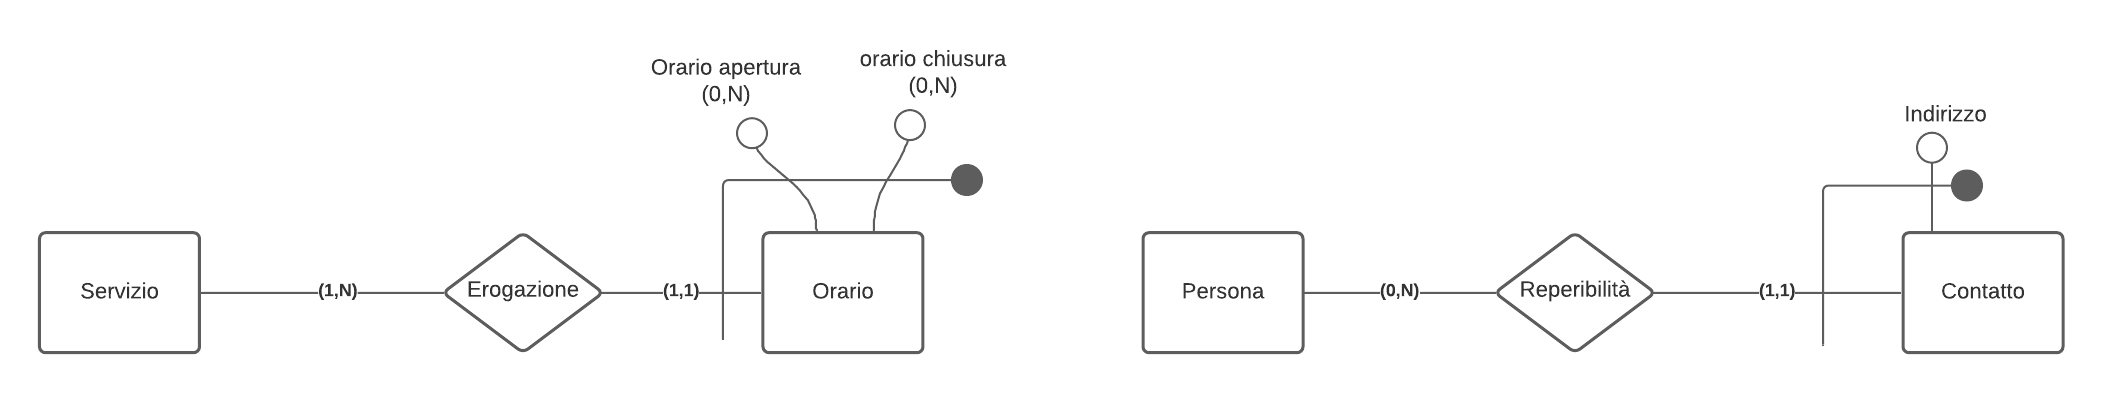
\includegraphics[width=\linewidth / 2]{img/multi_valore.png}
\end{center}


\subsection{Eliminazione delle generalizzazioni}

\paragraph{Cliente}\mbox{}\\
Si accorpano Cliente abituale e cliente occasionale a Cliente. Dato che la quantità di soste è un attributo utile per entrambe le tipologie di cliente. Lo sconto personale sarà invece impostato ad un valore che indica la percentuale di sconto se il cliente è abituale e a NULL se il cliente è occasionale.

\paragraph{Persona}\mbox{}\\
Nelle generalizzazioni di persona, per evitare inutili valori NULL in un eventuale accorpamento \textbf{Persona} viene mantenuta come entità. Questa entità conterrà tutti i dati relativi alla persona e avrà due entità deboli collegate ovvero \textbf{Addetto} e \textbf{Cliente}.

Persona avrà da 0 a 1 \textbf{Cliente} e da 0 a 1 \textbf{Addetto}. Chiaramente ogni \textbf{Cliente}  e \textbf{Addetto} avrà una e una sola persona legata. In \textbf{Addetto} e \textbf{Cliente} posizioneremo i dati relativi a queste due entità come da schema concettuale.

\subsection{Modifiche, aggiunte e chiarimenti alle chiavi}

Tutte le chiavi primarie sono definite utilizzando le chiavi della progettazione concettuale, tranne nei seguenti casi.

\paragraph{Imbarcazione} Ad \textbf{Imbarcazione} oltre alla sua chiave primaria Codice internazionale viene aggiunto un id autoincrementante utilizzato come chiave\footnote{Chiave unica}. Questo è stato scelto per poter utilizzare il costraint relativo alla sovrapposizione delle soste. Infatti esso funziona solo con attributi interi e non con Varchar\footnote{A meno di installare il pacchetto aggiuntivo di Postgres che lo permetta ma per lo scopo di questo progetto abbiamo preferito evitare per questioni di compatibilità.}.

\paragraph{Persona} A \textbf{Persona} oltre alla sua chiave primaria \textit{Codice fiscale} viene aggiunto un id autoincrementante utilizzato come chiave\footnote{Chiave unica}. Questo è stato scelto per poter utilizzare il costraint relativo alla sovrapposizione delle prenotazioni. Infatti esso funziona solo con attributi interi e non con Varchar.

\paragraph{Addetto} Addetto concettualmente eredita la chiave primaria di \textbf{Persona} ma come da progettazione concettuale mantiene la chiave su \underline{Servizio gestito, Data inizio contratto}. Come chiave primaria si sceglie quindi di utilizzare il \textit{codice fiscale} derivante da \textbf{persona} perché più leggero.

\paragraph{Periodo di apertura} Per ridurre lo spazio utilizzato nella tabella che rappresenta la relazione \textit{Apertura}, a \textbf{Periodo di apertura} abbiamo aggiunto una chiave primaria tramite id autoincrementante. Chiaramente non abbiamo rimosso la chiave unica già presente, infatti essa garantisce l'unicità delle triple presenti.




\subsection{Schema concettuale ristrutturato - Schema logico}
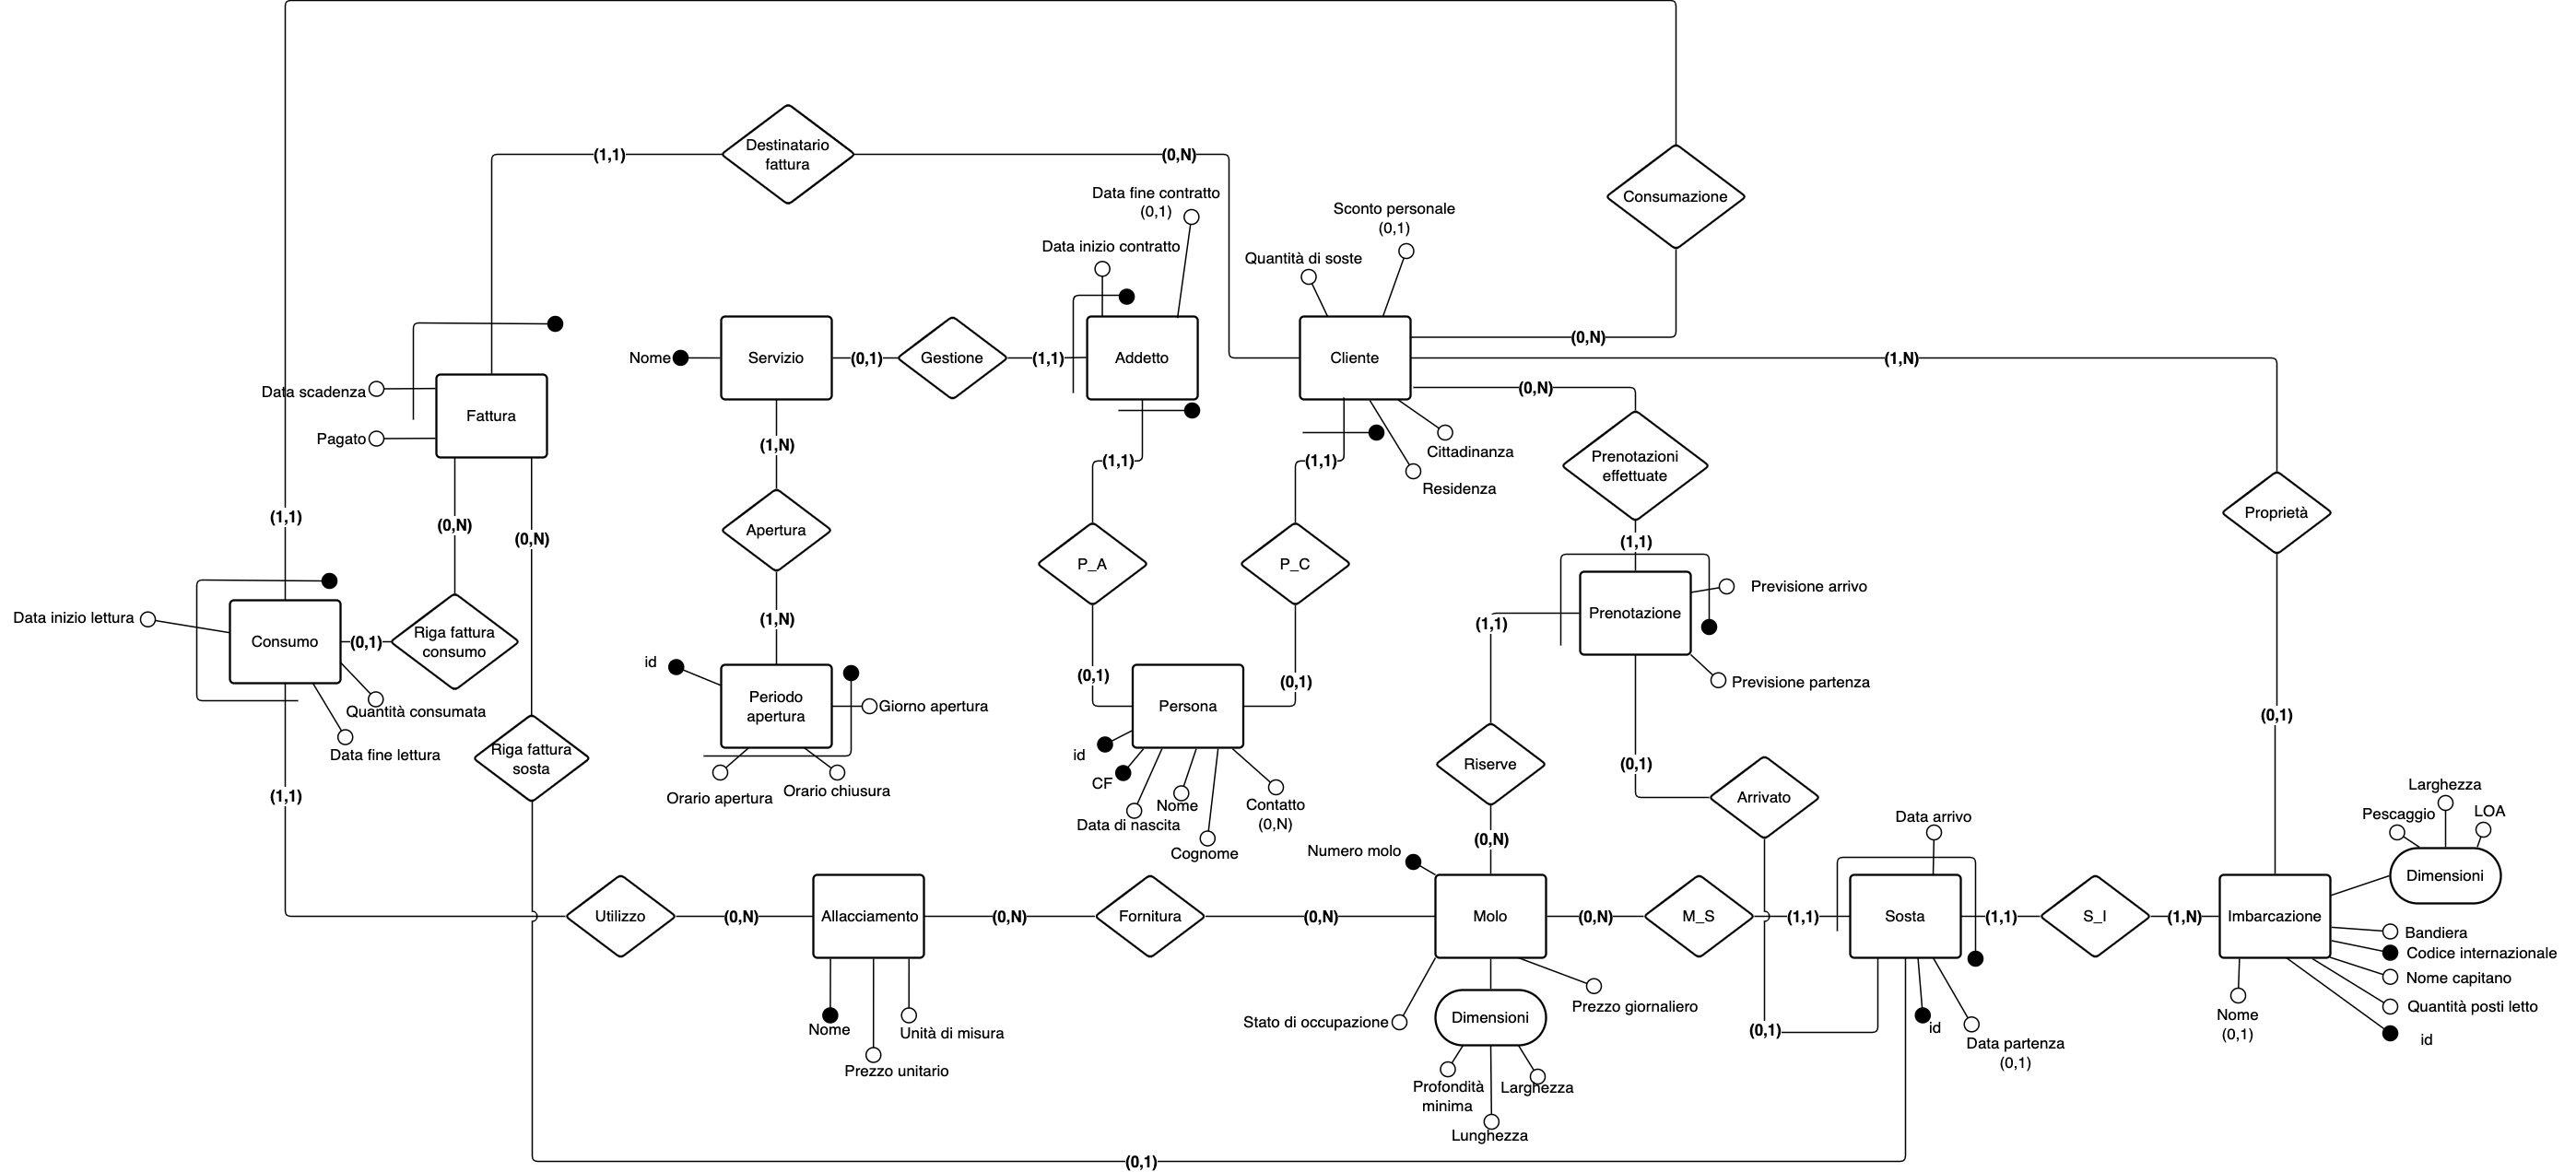
\includegraphics[width=\textwidth]{img/erlogico.png}


\subsection{Descrizione schema relazionale}

Per questione di compatibilità con il \textit{DBMS} alcuni nomi di attributi entità e relazioni sono stati normalizzati sostituendo gli spazi con underscore, togliendo gli accenti, accorciando i nomi molto lunghi e con altre piccole accortezze.

Imbarcazione(\underline{codice\_internazionale}, bandiera, nome capitano, qtpostiletto, nome, dimensioni, pescaggio, larghezza, LOA);

Molo(\underline{numero molo}, stato di occupazione,dimensioni, profondità minima, larghezza, lunghezza);

Servizio(\underline{nome del servizio});

Addetto(\underline{servizio}, \underline{Servizio, data\_inizio \_contratto}, data\_fine\_contratto);

Cliente (cittadinanza, residenza);

Cliente occasionale(quantità\_sosta);

Cliente abituale (sconto\_personale);

Persona(\underline{CF},data di nascita, nome, cognome, contatto);

Prenotazione(\underline{cf, id, previsione arrivo, molo}  previsione\_partenza);

Sosta (\underline{imbarcazione, molo,data\_arrivo,} data partenza);

Allacciamento(\underline{nome, prezzo\_unitario, unita\_di misura});

Periodo di apertura (\underline{giorno\_apertura,orario\_apertura, orario\_chiusura});


Consumo(\underline{cliente, allaciamento, data inizio lettura}, data fine lettura, quantità consumata);

Fattura(\underline{fattura, data\_scadenza}, pagato); 



La chiave primaria è la prima delle chiavi indicate dalla sottilineatura.

\subsection{Check e costraint}



\subsection{Vincoli di integrità referenziali}

\textbf{Fattura}.cliente -> Cliente.persona\\
\textbf{Addetto}.persona -> Persona.CF\\
\textbf{Cliente}.persona -> Persona.CF\\
\textbf{Molo}.dimensioni -> dimensioni.id\_dimensioni\\
\textbf{Imbarcazione}.dimensioni -> dimensioni.id\_dimensioni\\
\textbf{Servizio}.marina -> Marina.coordinate geografiche\\
\textbf{Contatto}.persona -> Persona.CF\\
\textbf{Orario}.servizio ->Servizio.nome\\
\textbf{Orario}.marina -> Marina.coordinate\_geografiche\\
\textbf{Fattura}.consumo -> Consumo.id\_consumo\\
\textbf{Consumo}.marina -> Marina.coordinate\_geografiche\\
\textbf{Servizio}.addetto -> Addetto.persona\\
\textbf{Prenotazione}.molo -> Molo.id\_molo\\
\textbf{Molo}.marina -> Marina.coordinate\_geografiche\\

%\section{Casistiche di utilizzo della base di dati}

%-	Quando un utente va via dovrà quindi pagare il conto, che è la somma di tutti i servizi di cui ha usufruito
%-	Avere facilmente in vista tutte le persone all’interno del marina
%-	Conoscere rapidamente quanti posti disponibili relativamente a certe dimensioni ci sono
%-	Ottenere i dati necessari a compilare i documenti doganali e relativi al soggiorno in uno stato estero per gli utenti con nazionalità differente dal marina


\section{Query}

\subsection{Classifica clienti più spendenti}
\subsection{Entrate di ogni anno divise in ricevute e da ricevere}
\subsection{Quantità di moli di ogni marina}

\subsection{Moli disponibili in un certo periodo per determinate dimensioni di barca}

\begin{lstlisting}
SELECT idmolo,dimensioni,marina from "Molo"
--SELECT count(idmolo) from "Molo"
JOIN "Dimensioni" d on d.id_dimensioni = "Molo".dimensioni

WHERE idmolo not in (
SELECT molo FROM "sosta"
WHERE data_arrivo<='2022-01-20 22:16:37.000000'
AND '2022-12-26 8:16:37.000000' <= data_partenza)

AND idmolo not in (
SELECT molo FROM "Prenotazione"
WHERE previsione_arrivo<='2022-01-20 22:16:37.000000'
AND '2022-12-26 8:16:37.000000' <= previsione_partenza)

AND lunghezza >= 9 and larghezza>= 3 and pescaggio >= 3
AND marina = '{45.47186543638522000,12.44861260105955800}'
ORDER BY dimensioni ASC;
LIMIT 10;
\end{lstlisting}

\subsection{Tutte le soste fatte dall'imbarcazione "Alexandra"}

Tutte le soste effettuate dall'imbarcazione "Alexandra" in uno dei marina ed in che date è arrivata in quel marina

\begin{lstlisting}
SELECT Mar.nome, I.nome, sosta.data_arrivo  FROM sosta
JOIN "Imbarcazione"  I on sosta.imbarcazione = I.codice_internazionale
JOIN "Molo" M on M.idmolo = sosta.molo
JOIN "Marina" Mar on M.marina = Mar.coordinate_geografiche

WHERE I.nome = 'Alexandra';
\end{lstlisting}

\subsection{Clienti con barca norvegese che hanno sostato a Portoferraio nel 2022}

\begin{lstlisting}
SELECT DISTINCT P.nome,P.cognome FROM sosta
JOIN "Imbarcazione" I on I.codice_internazionale = sosta.imbarcazione
JOIN "Molo" M on M.idmolo = sosta.molo
JOIN "Marina" mar on M.marina = mar.coordinate_geografiche
JOIN "Cliente" C on I.proprietario = C.persona
JOIN "Persona" P on C.persona = P.cf
WHERE data_arrivo>= '2022-01-01 00:00:00.000000'
AND data_partenza <= '2022-12-31 00:00:00.000000'
AND I.bandiera = 'Norvegia'
AND mar.citta = 'Portoferraio';
\end{lstlisting}

\section{Indicizzazione}

Essendo modificata pochissime volte\footnote{Ovvero solo in caso di ristrutturazioni del marina} e letta spesso in moltissime operazioni, l'entità \textbf{Molo} è importante che venga indicizzata tramite B-Tree, in questo modo, entrando per mezzo dell'id sarà decisamente più efficiente leggerne attributi come ad esempio le dimensioni o lo stato di occupazione.

L'indice appena descritto sarebbe poi comunque utile anche in caso di utilizzo su larga scala con migliaia di moli, oppure nel caso si volesse adattare la base dati all'utilizzo con una serie marina contenenti molti moli. I risultati di efficienza aumentata sarebbero quindi ancora più evidenti e utili.

Sono stati poi, come precedentemente descritto al punto \ref{vincoli_gestiti} , utilizzati dei search tree per utilizzare al meglio i costraint relativi alle date ed orari di \textbf{prenotazioni} e \textbf{soste}.


\end{document}
